\section{Related work}
\subsection{SKEP}

SKEP \cite{DBLP:journals/corr/abs-2005-05635}, or the Sentiment Knowledge Enhanced Pre-training model, is a deep learning architecture developed by PaddlePaddle, which uses an unsupervised pre-training process and a supervised fine-tuning process to achieve high accuracy in various NLP tasks, including sentiment analysis.

In this project, we utilized the SKEP model to encode the text data and classify the sentiment polarity of each attribute. Specifically, we fine-tuned the pre-trained SKEP model on our labeled dataset to classify the sentiment polarity of each attribute. By leveraging the strengths of the SKEP model, we were able to achieve high accuracy in both opinion extraction and relation classification tasks.

One advantage of using the SKEP model is its ability to capture long-term dependencies and semantic information in text data. This is achieved through the use of a transformer-based architecture, which allows for efficient encoding of sequences of text data. Additionally, the SKEP model utilizes a self-attention mechanism, which enables it to attend to different parts of the input text when generating output representations, allowing it to capture the most important information in the input.

% insert picture SKEP model
\begin{figure}
    \centering
    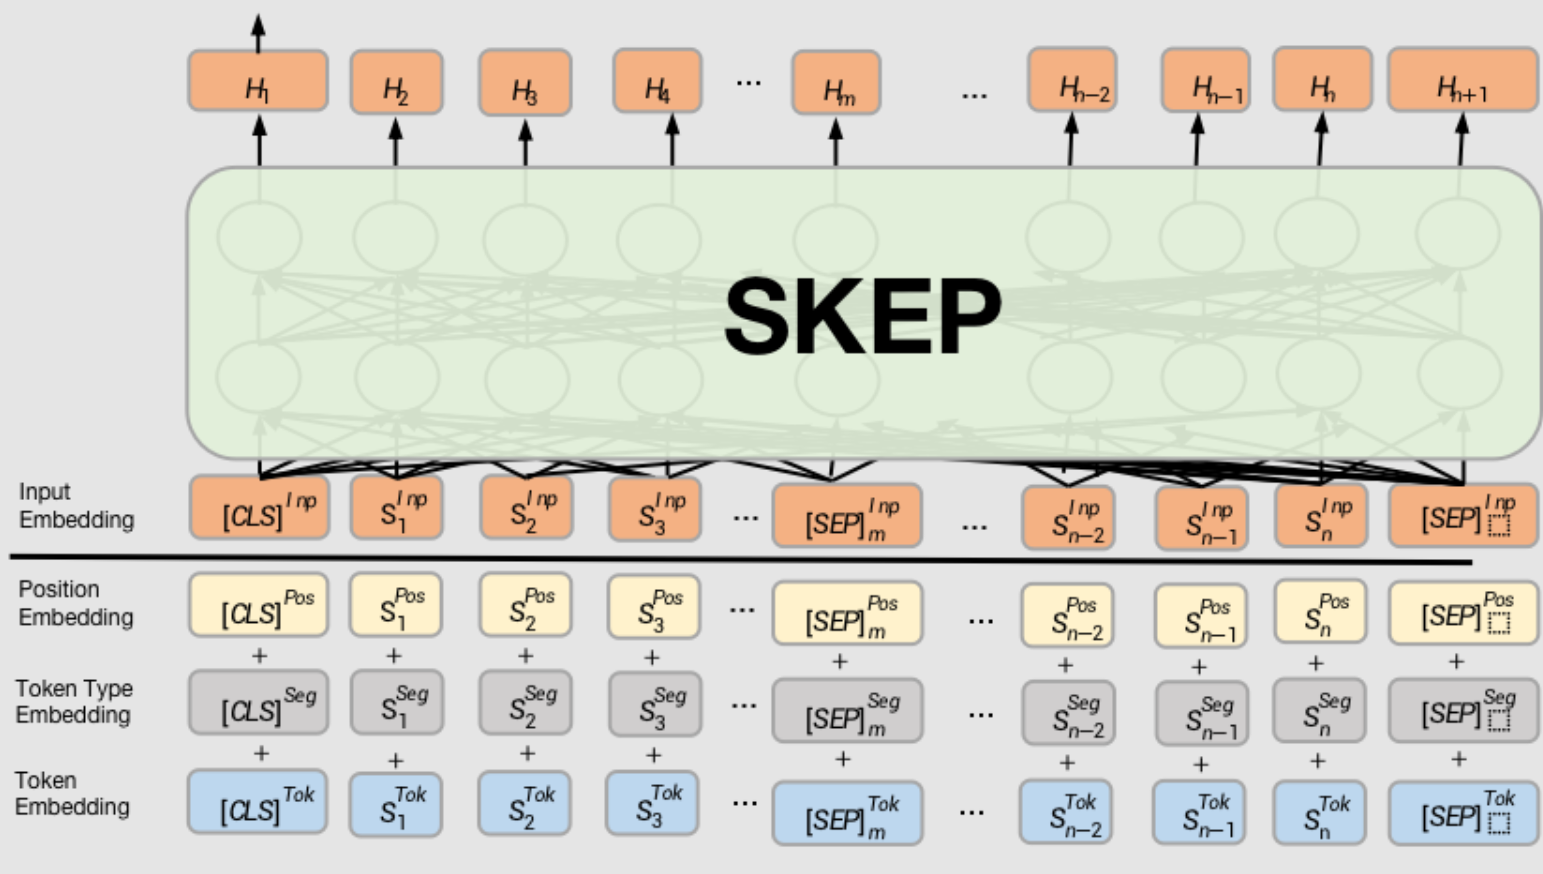
\includegraphics[width=0.8\textwidth]{SKEP.png}
    \caption{SKEP model}
    \label{fig:SKEP}
\end{figure}

\subsection{Opener}

Opener is a dataset developed by SemEval-2022 Task 10, which contains subjective text data from various domains, including social media, product reviews, and customer feedback. The dataset is annotated with attributes and corresponding opinions, which can be used to train models for opinion extraction and relation classification tasks.

% insert picture Dataset
\begin{figure}
    \centering
    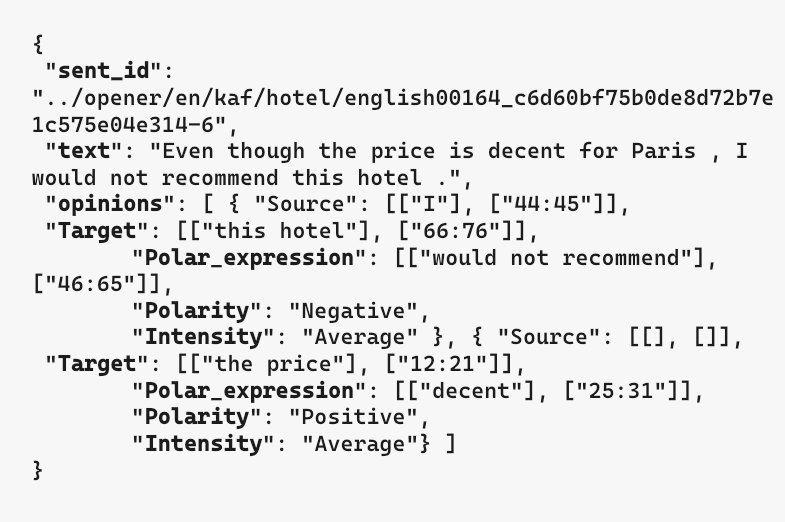
\includegraphics[width=0.8\textwidth]{Dataset.png}
    \caption{Opener Dataset}
    \label{fig:Dataset}
\end{figure}

\subsection{Sequence Lebeling Pipeline}

Another relevant piece of related work is the starter code provided by SemEval-2022 Task 10, which is focused on extracting sentiment relations from customer reviews.

The system first uses three separate BiLSTM models to extract holders, targets, and expressions from the text. These sub-elements are then passed to a relation prediction model, which creates contextualized representations of the full text, the first element (holder or target), and the sentiment expression using a BiLSTM and max pooling.

The representations are concatenated and passed through a linear layer followed by a sigmoid function to predict whether two elements have a relationship or not. The training involves binary classification of relationship prediction.

During inference, the system predicts all sub-elements and then decides if they have a relationship based on a threshold (prediction > 0.5). The predictions are then converted to the json format used in the shared task.

While this system is specifically designed for SemEval-2022 Task 10, it provides an example of a pipeline approach for sentiment relation extraction, using both sequence labeling and relation prediction models. This approach has the potential to be applied to other domains and datasets for structured sentiment analysis tasks.
